%%%%%%%%%
%%%%%%%%%%
%%%%%%%%%%%
%%%%%%%%%%%%
%%%%%%%%%%%%%

\begin{figure}[t]
\centering

% ----------------- Top row -----------------
\begin{minipage}{0.3\linewidth}
\centering
\pgfplotsset{set layers}
\begin{tikzpicture}
\begin{axis}[
    width=\linewidth,
    height=1.2\linewidth,
    xlabel={Number of MPI ranks},
    ylabel={Time (s)},
    ymode=log,
    xmode=log,
    xtick={16,36,64,100},
    % ----- FORCE TICKS -----
    xtick={16,36,64,100},
    xticklabels={64,144,256,400},
    ytick={100,200,400,800},
    yticklabels={100,200,400,800},  
    scaled x ticks=false,
    scaled y ticks=false,
    title={All: Time},
    tick label style={font=\small},
    label style={font=\small},
    axis line style={black, line width=1pt},
    grid=major,
    grid style={dashed, gray!30},
    line width=1pt
]
    \addplot+[mark=o, solid, mark size=2pt, blue] coordinates {(16,530) (36,255) (64,174) (100,117.5)};
    \addplot+[mark=o, dashed, mark size=2pt, blue] coordinates {(16,570.9) (36,288.1) (64,215.2) (100,147.8)};
    % Upper CI curve
    \addplot[
        name path=upper,
        draw=none
    ] coordinates {
        (16,534) (36,258) (64,177) (100,124)
    };

    % Lower CI curve
    \addplot[
        name path=lower,
        draw=none
    ] coordinates {
        (16,526) (36,252) (64,171) (100,110)
    };

    % Confidence band
    \addplot[
        blue!20
    ] fill between[
        of= lower and upper,
    ];
    
    \addplot[
        name path=upper2,
        draw=none
    ] coordinates {
        (16,579) (36,294) (64,210) (100,152)
    };

    % Lower CI curve
    \addplot[
        name path=lower2,
        draw=none
    ] coordinates {
        (16,561) (36,282) (64,220) (100,143)
    };

    % Confidence band
    \addplot[
        blue!20
    ] fill between[
        of=lower2 and upper2,
    ];
    
% Ideal case line
\addplot[
    black,
    dash dot,
    no markers,
    line width=1pt
] coordinates {
    (16,450)
    (36,200)
    (64,112.5)
    (100,72)
};
\node at (axis cs:86,70) [anchor=south east, black, font=\small] {Ideal};
\end{axis}
\end{tikzpicture}
\end{minipage}
\hfill
\begin{minipage}{0.3\linewidth}
\pgfplotsset{set layers}
\centering
\begin{tikzpicture}
\begin{axis}[
    width=\linewidth,
    height=1.2\linewidth,
    xlabel={Number of MPI ranks},
    ylabel={Time (s)},
    xmode=log,
    ymode=log,
    % ----- FORCE TICKS -----
    xtick={16,36,64,100},
    xticklabels={64,144,256,400},
    ytick={300,600,1200,2400},
    yticklabels={300,600,1200, 2400},    
    scaled x ticks=false,
    scaled y ticks=false,
    title={All: Time},
    tick label style={font=\small},
    label style={font=\small},
    grid=major,
    axis line style={black, line width=1pt},
    grid style={dashed, gray!30},
    line width=1pt
]
    % Upper CI curve
    \addplot[
        name path=upper,
        draw=none
    ] coordinates {
        (16,1145) (36,575) (64,400) (100,300)
    };

    % Lower CI curve
    \addplot[
        name path=lower,
        draw=none
    ] coordinates {
        (16,1135) (36,565) (64,380) (100,290)
    };

    % Confidence band
    \addplot[
        red!20
    ] fill between[
        of=upper and lower,
    ];
    
    \addplot[
        name path=upper2,
        draw=none
    ] coordinates {
        (16,1185) (36,640) (64,455) (100,365)
    };

    % Lower CI curve
    \addplot[
        name path=lower2,
        draw=none
    ] coordinates {
        (16,1175) (36,634) (64,439) (100,357)
    };

    % Confidence band
    \addplot[
        red!20
    ] fill between[
        of=upper2 and lower2,
    ];

    \addplot[
        name path=upper3,
        draw=none
    ] coordinates {
        (16,1900) (36,1049) (64,810) (100,703)
    };

    % Lower CI curve
    \addplot[
        name path=lower3,
        draw=none
    ] coordinates {
        (16,1880) (36,1047) (64,808) (100,701)
    };

    % Confidence band
    \addplot[
        green!20
    ] fill between[
        of=upper3 and lower3,
    ];

    \addplot[
        name path=upper4,
        draw=none
    ] coordinates {
        (16,1915) (36,1192) (64,866) (100,760)
    };

    % Lower CI curve
    \addplot[
        name path=lower4,
        draw=none
    ] coordinates {
        (16,1905) (36,1188) (64,860) (100,750)
    };

    % Confidence band
    \addplot[
        green!20
    ] fill between[
        of=upper4 and lower4,
    ];
    
%\addplot+[mark=o, solid, mark size=2pt, blue] coordinates {(16,450.9) (36,275.1) (64,151.2) (100,105.8)};
%\addplot+[mark=o, dashed, mark size=2pt, blue] coordinates {(16,487.4) (36,316.1) (64,181.1) (100,129.4)};
\addplot+[mark=square, solid, mark size=2pt, red] coordinates {(16,1140) (36,570) (64,390) (100,295)};
\addplot+[mark=square, dashed, mark size=2pt, red] coordinates {(16,1180) (36,637) (64,452) (100,361)};
\addplot+[mark=triangle, solid, mark size=2pt, green!60!black] coordinates {(16,1890) (36,1048) (64,809) (100,702)};
\addplot+[mark=triangle, dashed, mark size=2pt, green!60!black] coordinates {(16,1910) (36,1190) (64,863) (100,755)};
% Ideal case line
\addplot[
    black,
    dash dot,
    no markers,
    line width=1pt
] coordinates {
    (16,1600)
    (36,711)
    (64,400)
    (100,256)
};
\node at (axis cs:82,640) [anchor=south east, black, font=\small] {Ideal};
\end{axis}
\end{tikzpicture}
\end{minipage}
\hfill
\begin{minipage}{0.3\linewidth}
\pgfplotsset{set layers}
\centering
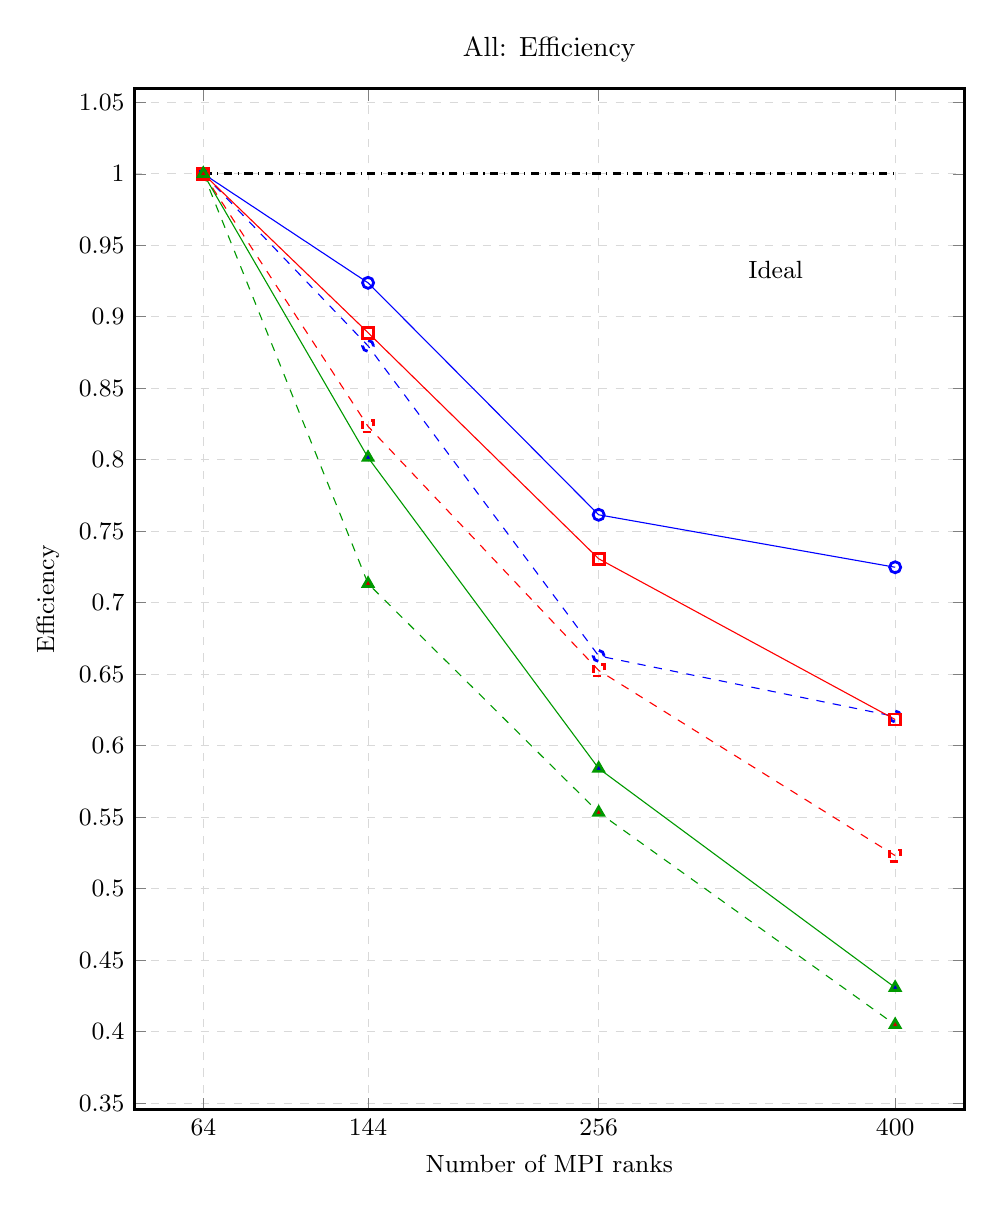
\begin{tikzpicture}
\begin{axis}[
    width=\linewidth,
    height=1.2\linewidth,
    xlabel={Number of MPI ranks},
    ylabel={Efficiency},
    xtick={16,36,64,100},
    xticklabels={64,144,256,400},
    title={All: Efficiency},
    tick label style={font=\small},
    label style={font=\small},
    grid=major,
    axis line style={black, line width=1pt},
    grid style={dashed, gray!30},
    line width=1pt
]

\addplot+[mark=o, solid, mark size=2pt, blue] coordinates {(16,1.0000) (36,530*16/255/36) (64,530*16/174/64) (100,530*16/117/100)};
\addplot+[mark=o, dashed, mark size=2pt, blue] coordinates {(16,1.0000) (36,570*16/288/36) (64,570*16/215/64) (100,570*16/147/100)};
\addplot+[mark=square, solid, mark size=2pt, red] coordinates {(16,1.0000) (36,1140*16/570/36) (64,1140*16/390/64) (100,1140*16/295/100)};
\addplot+[mark=square, dashed, mark size=2pt, red] coordinates {(16,1.0000) (36,1180*16/637/36) (64,1180*16/452/64) (100,1180*16/361/100)};
\addplot+[mark=triangle*, solid, mark size=2pt, green!60!black] coordinates {(16,1.0000) (36,1890*16/1048/36) (64,1890*16/809/64) (100,1890*16/702/100)};
\addplot+[mark=triangle*, dashed, mark size=2pt, green!60!black] coordinates {(16,1.0000) (36,1910*16/1190/36) (64,1910*16/863/64) (100,1910*16/755/100)};
\addplot[
    black,
    dash dot,
    no markers,
    line width=1pt
] coordinates {
    (16,1)
    (36,1)
    (64,1)
    (100,1)
};
\node at (axis cs:90,0.92) [anchor=south east, black, font=\small] {Ideal};
\end{axis}
\end{tikzpicture}
\end{minipage}

\vspace{1em}

% ----------------- Bottom row -----------------
\begin{minipage}{0.3\linewidth}
\pgfplotsset{set layers}
\centering
\begin{tikzpicture}
\begin{axis}[
    width=\linewidth,
    height=1.2\linewidth,
    xlabel={Number of MPI ranks},
    ylabel={Time (s)},
    ymode=log,
    xmode=log,
    xtick={4,6,8,10},
    xticklabels={8,12,16,20},
    ytick={5,10,20,40},
    yticklabels={5,10,20,40},      
    title={QR: Time},
    tick label style={font=\small},
    label style={font=\small},
    grid=major,
    axis line style={black, line width=1pt},
    grid style={dashed, gray!30},
    line width=1pt
]
\addplot+[mark=o, solid, mark size=2pt, blue] coordinates {(4,19) (6,14) (8,11.2) (10,9.2)};
\addplot+[mark=o, dashed, mark size=2pt, blue] coordinates {(4,53) (6,43) (8,41) (10,38)};

    % Upper CI curve
    \addplot[
        name path=upper,
        draw=none
    ] coordinates {
        (4,22) (6,14.5) (8,12) (10,9.5)
    };

    % Lower CI curve
    \addplot[
        name path=lower,
        draw=none
    ] coordinates {
        (4,16) (6,13.5) (8,10) (10,8.9)
    };

    % Confidence band
    \addplot[
        blue!20
    ] fill between[
        of= lower and upper,
    ];
    
    \addplot[
        name path=upper2,
        draw=none
    ] coordinates {
        (4,56) (6,46) (8,43) (10,40)
    };

    % Lower CI curve
    \addplot[
        name path=lower2,
        draw=none
    ] coordinates {
        (4,50) (6,40) (8,38) (10,36)
    };

    % Confidence band
    \addplot[
        blue!20
    ] fill between[
        of=lower2 and upper2,
    ];
    
\addplot[
    black,
    dash dot,
    no markers,
    line width=1pt
] coordinates {
    (4,33)
    (6,22)
    (8,16.5)
    (10,13.2)
};
\node at (axis cs:9.9,18) [anchor=south east, black, font=\small] {Ideal};
\end{axis}
\end{tikzpicture}
\end{minipage}
\hfill
\begin{minipage}{0.3\linewidth}
\pgfplotsset{set layers}
\centering
\begin{tikzpicture}
\begin{axis}[
    width=\linewidth,
    height=1.2\linewidth,
    xlabel={Number of MPI ranks},
    ylabel={Time (s)},
    ymode=log,
    xmode=log,
    xtick={4,6,8,10},
    xticklabels={8,12,16,20},
    ytick={20,40,80,160},
    yticklabels={20,40,80,160},  
    title={QR: Time},
    tick label style={font=\small},
    label style={font=\small},
    grid=major,
    axis line style={black, line width=1pt},
    grid style={dashed, gray!30},
    line width=1pt
]
\addplot+[mark=square, solid, mark size=2pt, red] coordinates {(4,75) (6,57) (8,46) (10,36)};
\addplot+[mark=square, dashed, mark size=2pt, red] coordinates {(4,127) (6,103) (8,91.8) (10,86.3)};
\addplot+[mark=triangle, solid, mark size=2pt, green!60!black] coordinates {(4,198) (6,150) (8,124) (10,100)};
\addplot+[mark=triangle, dashed, mark size=2pt, green!60!black] coordinates {(4,223) (6,178) (8,156) (10,146)};

    % Upper CI curve
    \addplot[
        name path=upper,
        draw=none
    ] coordinates {
        (4,78) (6,59) (8,48) (10,37)
    };

    % Lower CI curve
    \addplot[
        name path=lower,
        draw=none
    ] coordinates {
        (4,72) (6,55) (8,44) (10,35)
    };

    % Confidence band
    \addplot[
        red!20
    ] fill between[
        of=upper and lower,
    ];
    
    \addplot[
        name path=upper2,
        draw=none
    ] coordinates {
        (4,127) (6,103) (8,92) (10,87)
    };

    % Lower CI curve
    \addplot[
        name path=lower2,
        draw=none
    ] coordinates {
        (4,127) (6,103) (8,91.6) (10,85.6)
    };

    % Confidence band
    \addplot[
        red!20
    ] fill between[
        of=upper2 and lower2,
    ];

    \addplot[
        name path=upper3,
        draw=none
    ] coordinates {
        (4,200) (6,155) (8,126) (10,102)
    };

    % Lower CI curve
    \addplot[
        name path=lower3,
        draw=none
    ] coordinates {
        (4,196) (6,145) (8,122) (10,98)
    };

    % Confidence band
    \addplot[
        green!20
    ] fill between[
        of=upper3 and lower3,
    ];

    \addplot[
        name path=upper4,
        draw=none
    ] coordinates {
        (4,223) (6,179) (8,157) (10,146)
    };

    % Lower CI curve
    \addplot[
        name path=lower4,
        draw=none
    ] coordinates {
        (4,223) (6,177) (8,155) (10,146)
    };

    % Confidence band
    \addplot[
        green!20
    ] fill between[
        of=upper4 and lower4,
    ];
    
\addplot[
    black,
    dash dot,
    no markers,
    line width=1pt
] coordinates {
    (4,120)
    (6,80)
    (8,60)
    (10,48)
};
\node at (axis cs:9.9,40) [anchor=south east, black, font=\small] {Ideal};
\end{axis}
\end{tikzpicture}
\end{minipage}
\hfill
\begin{minipage}{0.3\linewidth}
\centering
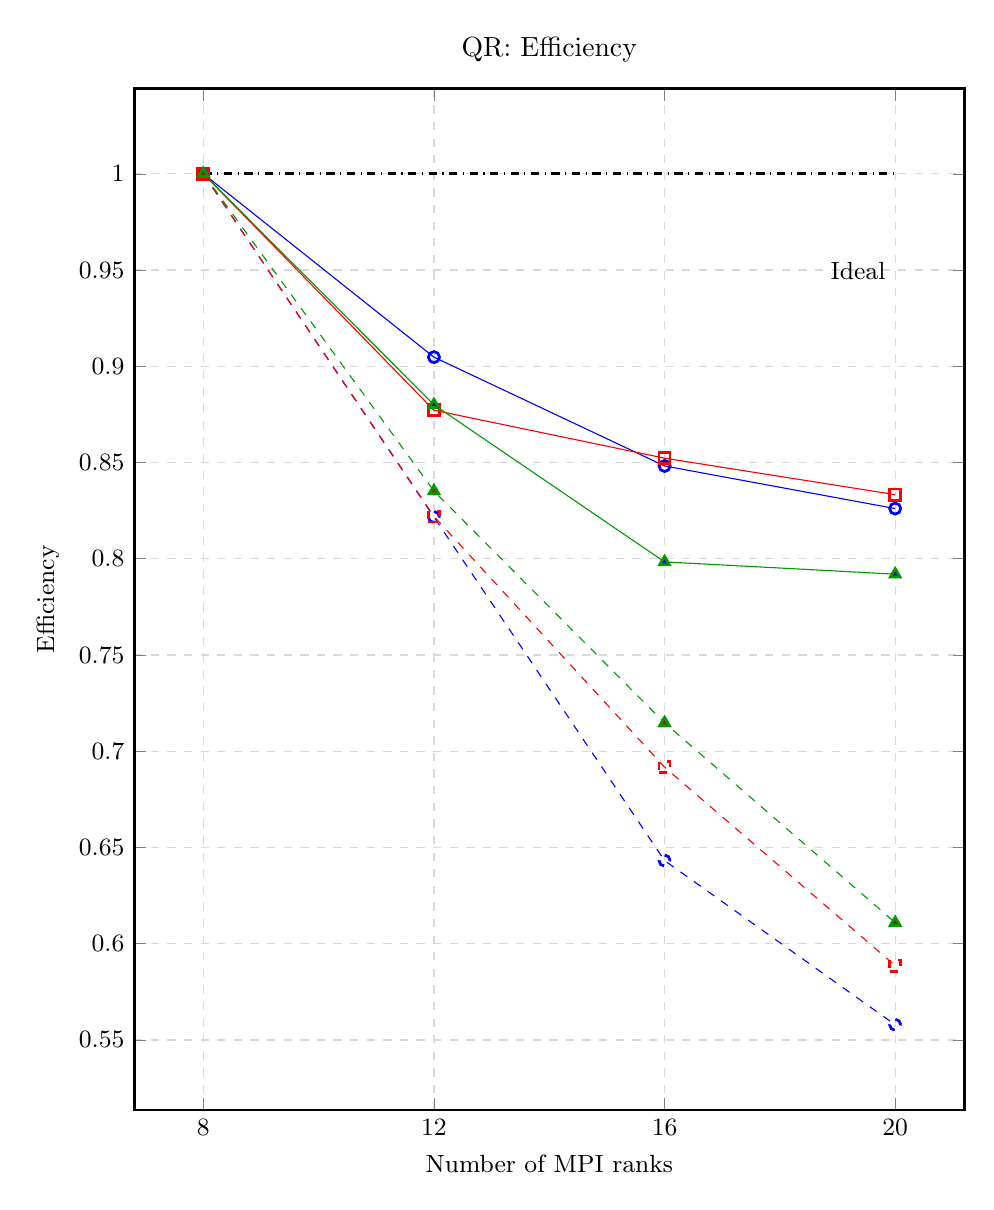
\begin{tikzpicture}
\begin{axis}[
    width=\linewidth,
    height=1.2\linewidth,
    xlabel={Number of MPI ranks},
    ylabel={Efficiency},
    xtick={4,6,8,10},
    xticklabels={8,12,16,20},
    title={QR: Efficiency},
    tick label style={font=\small},
    label style={font=\small},
    grid=major,
    axis line style={black, line width=1pt},
    grid style={dashed, gray!30},
    line width=1pt
]

\addplot+[mark=o, solid, mark size=2pt, blue] coordinates {(4,1.0000) (6,19*4/6/14) (8,19*4/8/11.2) (10,19*4/10/9.2)};
\addplot+[mark=o, dashed, mark size=2pt, blue] coordinates {(4,1.0000) (6,53*4/6/43) (8,53*4/8/41.2) (10,53*4/10/38)};
\addplot+[mark=square, solid, mark size=2pt, red] coordinates {(4,1.0000) (6,75*4/6/57) (8,75*4/8/44) (10,75*4/10/36)};
\addplot+[mark=square, dashed, mark size=2pt, red] coordinates {(4,1.0000) (6,127*4/6/103) (8,127*4/8/91.8) (10,127*4/10/86.3)};
\addplot+[mark=triangle*, solid, mark size=2pt, green!60!black] coordinates {(4,1.0000) (6,198*4/6/150) (8,198*4/8/124) (10,198*4/10/100)};
\addplot+[mark=triangle*, dashed, mark size=2pt, green!60!black] coordinates {(4,1.0000) (6,223*4/6/178) (8,223*4/8/156) (10,223*4/10/146)};
\addplot[
    black,
    dash dot,
    no markers,
    line width=1pt
] coordinates {
    (4,1)
    (6,1)
    (8,1)
    (10,1)
};
\node at (axis cs:10,0.94) [anchor=south east, black, font=\small] {Ideal};
\end{axis}
\end{tikzpicture}
\end{minipage}

% ----------------- Shared legend below all plots -----------------
\vspace{1em}
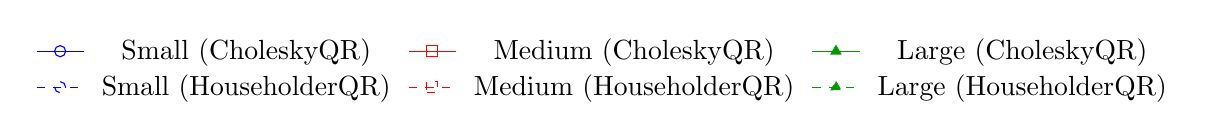
\begin{tikzpicture}
\begin{axis}[
    hide axis,
    xmin=0, xmax=1,
    ymin=0, ymax=1,
    legend columns=3,
    legend style={
        draw=none,
        column sep=1ex
    }
]
% define legend entries without plotting points
\addlegendimage{mark=o, solid, blue}
\addlegendimage{mark=square, solid, red}
\addlegendimage{mark=triangle*, solid, green!60!black}
\addlegendimage{mark=o, dashed, blue}
\addlegendimage{mark=square, dashed, red}
\addlegendimage{mark=triangle*, dashed, green!60!black}

\legend{
Small (CholeskyQR),
Medium (CholeskyQR),
Large (CholeskyQR),
Small (HouseholderQR),
Medium (HouseholderQR),
Large (HouseholderQR)
}
\end{axis}
\end{tikzpicture}

\caption{Strong-scaling performance and parallel efficiency comparison between CholeskyQR and Householder QR across configurations. Each measurement was repeated five times. Runtime plots show the average execution time, with shaded bands indicating the minimum–maximum range across runs. Parallel efficiency is computed from the averaged runtimes.}
\label{fig:combined_strong_scaling}
\end{figure}